\documentclass[letterpaper, 10 pt, conference]{ieeeconf}  % Comment this line out if you need a4paper

\IEEEoverridecommandlockouts                              % This command is only needed if 
                                                          % you want to use the \thanks command

\overrideIEEEmargins                                      % Needed to meet printer requirements.

% See the \addtolength command later in the file to balance the column lengths
% on the last page of the document

% The following packages can be found on http:\\www.ctan.org
\usepackage{graphics} % for pdf, bitmapped graphics files
\usepackage{epsfig} % for postscript graphics files
\usepackage{mathptmx} % assumes new font selection scheme installed
\usepackage{times} % assumes new font selection scheme installed
\usepackage{amsmath} % assumes amsmath package installed
\usepackage{amssymb}  % assumes amsmath package installed
\usepackage{placeins}
\usepackage{hyperref}
\usepackage{bm}
\usepackage{float}

\usepackage[sorting=none]{biblatex}
\addbibresource{egbib.bib}

\DeclareMathOperator{\Ad}{\operatorname{Ad}}% Adjoint
\newcommand{\pd}[2]{\frac{\partial #1}{\partial #2}} % partial derivatives

\title{\LARGE \bf
Terrain-Aided Proprioceptive Localization for Snake Robots
}

\author{Riley Bridges, Quintin Dwight, Christian Foreman, and Andrew Scheffer%
}

\begin{document}

\maketitle
\thispagestyle{empty}
\pagestyle{empty}

\begin{abstract}
    In this report, our team presents a hybrid estimation scheme for tracking the shape, orientation, and global position of a 9-link robotic snake. Tracking the global pose of the snake as a whole is difficult in part because its internal shape changes are used to locomote the body such that no part of the robot intuitively represents the robot's pose at all times. To tackle this problem, our team leverages the idea of a non-conventional ``virtual chassis frame" to represent the robot's body frame. Our estimation pipeline uses this convention by first running an Extended Kalman Filter (EKF) that estimates the orientation, acceleration, and angular velocity of the virtual chassis frame. In tandem, our pipeline runs a particle filter leveraging force sensors embedded in every link of the robot to predict the position of the virtual chassis in the world. To test our pipeline, we develop a thorough simulation environment in Pybullet \cite{pybullet} and evaluate the EKF and particle filter independently. Our open-source implementation and additional documentation can be found on our GitHub: \href{https://github.com/schefferac2020/SnakeSim}{https://github.com/schefferac2020/SnakeSim}
\end{abstract}

\section{Introduction}

With recent advances in the field of biologically-inspired robotics, snake robots have drawn increased attention.  These hyper-redundant robotic mechanisms emulate the bodily structure of snakes being comprised of a sequence of interconnected links with kinematic constraints. The unique form factor of snake robots allow them to perform distinctive, adaptive, and versatile behavior in many different terrains. Hence, various snake-like robots have been proposed for various robotic tasks in extremely diverse environments such as underwater exploration and mapping \cite{underwater}, pipe inspection \cite{pipeline_inspection}, and even in the exploration of Saturn's moon, Enceladus \cite{enceladus}. 

In snake-like robot systems, the motion of the snake relies on complicated terrain contacts that span the entire body of the robot. For simplicity, one typically enforces a set of pre-determined sinusoidal motions called "gaits" that determine the motion of the individual robot joints with respect to time. Snake gaits rely on the effects of anisotropic friction between individual links and the terrain to propel the snake in a particular direction in the world frame. These gaits are incredibly useful in simplifying the control of hyper-redundant systems. 

Accomplishing an estimation of the 6DOF pose of each link of a snake-robot is a very difficult problem. In other robotic systems (i.e. robotic dogs, rovers, etc), the problem of estimating the position of the robot body is quite intuitive and typically involves tracking the motion of a stationary point on the robot across time. In the case of a snake-robot with an arbitrary number of links, however, no stationary point on the robot intuitively represents the ``pose" of the snake as a whole. In our snake system, we assume that each link is equipt with a unique Inertial Measurement Unit (IMU) and force-contact sensor. Additionally, we assume each joint has an absolute encoder. 

In this report, our team separates the snake-pose estimation problem into two components: 1) the estimation of the rotation, angular velocity, and acceleration of a ``virtual" body frame located at the snake's center of mass and aligned with the principle moments of inertia of the snake and 2) predicting the location of this body frame in the world frame using a particle filter based on contact-force sensors located on each link. We find that the ``virtual" body frame allows for intuitive and interpretable global motions of the snake. This paper overviews the effectiveness of our method in a custom PyBullet \cite{pybullet} simulation environment. 

\begin{figure}[H]
    \centering
    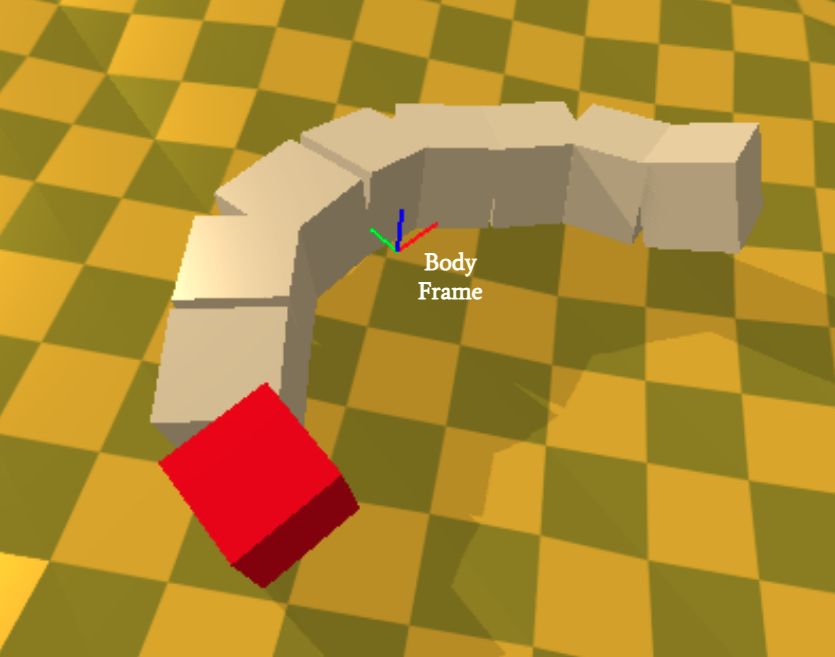
\includegraphics[width=0.85\linewidth]{sim_with_VC_frame.png}
    \caption{Our custom Pybullet simulation environment depicting a randomized mesh terrain, our 9-link snake, and its dynamic ``virtual" body frame}
    \label{fig:snake_overview}
\end{figure}

\section{Related Work}

The design and functionality of our hybrid estimation framework is built on many of the ideas in recent robotic-snake literature. Since the first robotic snake (developed in 1972 \cite{old_snakes}), numerous snake designs have been conceived and prototyped. As suggested in \cite{state_est_snake_robots}, a typical modular robotic snake configuration involves links with orthogonal joint axes, allowing the robot to perform cyclic movements (gaits) in three dimensions. A significant amount of effort has been conducted in the design of specific gaits that change the snake's pose with respect to the world frame in different ways. The idea is that by constraining the motion of the snake's joints, downstream estimation frameworks can take advantage of the movement characteristics that the gaits perform. For example, \cite{pipeline_inspection} developed a simple snake gait for traversing piping systems and was able to use the symmetry of this rolling gate to estimate an accurate position of the snake along the pipe and thus map the structure of the pipe over time.  

Building on the development of gaits, in \cite{state_est_snake_robots}, the authors constrain the motion of the snake robot to a simple "rolling" gait where the snake assumes a shape similar to the letter ``C" and continues to roll in a particular direction. This work pioneered the use of the ``virtual" body frame that we have chosen to use in this paper. The authors performed a study showcasing the effectiveness of the ``virtual" body frame. They did this by comparing the estimation error of an EKF tracking the orientation, angular velocity, and linear acceleration of a fixed-head frame (attached to the first link of the snake) and comparing it to an EKF tracking the corresponding quantities of the ``virtual" body frame. Overall, it was shown that the EKF operating on the virtual body allowed for a simple constant-velocity prediction step that performed well in the real world. Our method builds upon this method by simplifying the overall state tracked by the EKF and facilitating accurate position-localization in the world frame using a novel contact-based particle filter. 

\section{Methodology}
In this section, we will overview the robot model and movement gaits, a description of the ``virtual" body frame, our EKF prediction and update step, and the particle filter contact localization algorithm. 

\subsection{Snake Robot Definition}
In the figure below, we present the relevant frames of our simulated 9-link robotic snake platform. Note that the joints, represented by circles, alternate in rotating about the z-axis and the x-axis. 

\begin{figure}[H]
    \centering
    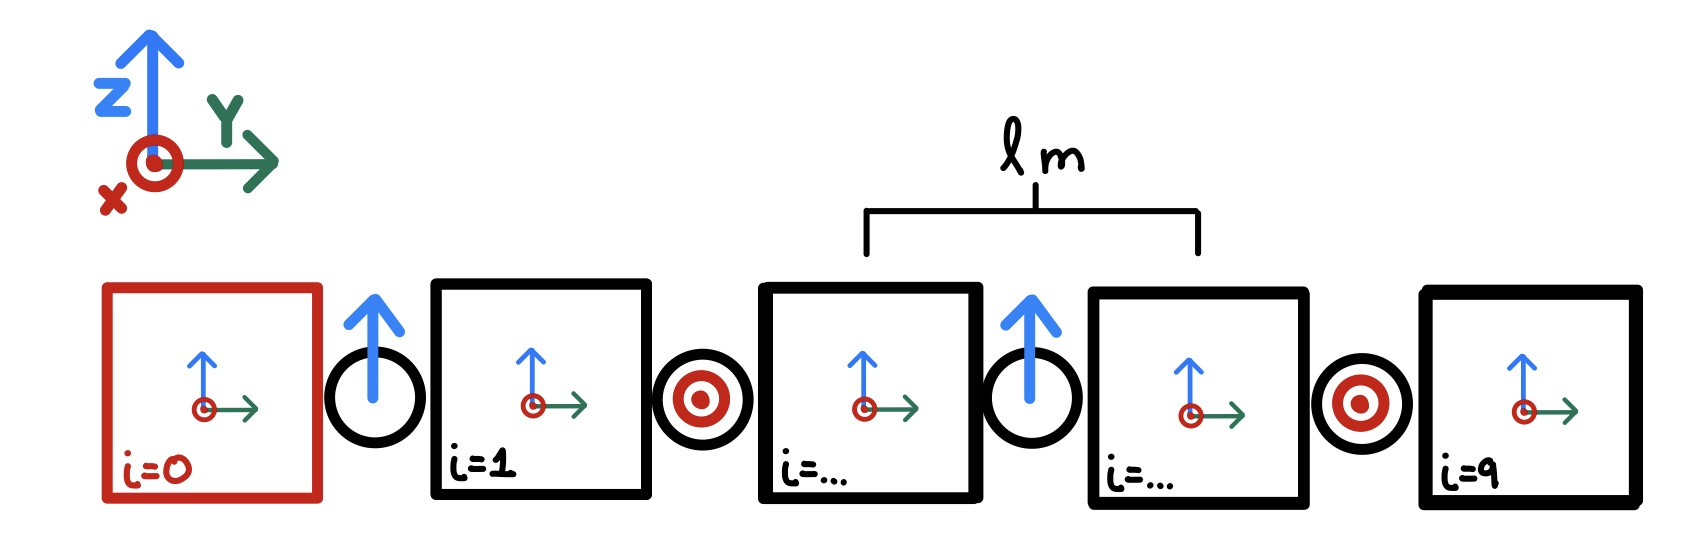
\includegraphics[width = 1\linewidth]{urdf.jpeg}
    \caption{Relevant link and joint frames of our snake URDF wrt the world}
    \label{fig:urdf}
\end{figure}

\noindent \textbf{Gate Equations}\\
Following \cite{state_est_snake_robots}, we utilize the following general gate equations to define the motion of the joints over time. Note that which gate equation is used is dependent on if the joint is "even" or "odd." In the following equation $\beta$, $A$ and $\delta$ are respectively the angular offset, amplitude, and phase shift between the even and odd joint waves. The component inside the sine functions describe the spatial frequency of the waves with respect to link number, i. 

\begin{equation}
    \theta(i, t) = \begin{cases} 
      \beta_{even} + A_{even}sin(\Omega_{even}i + \upsilon_{even}t)& \text{even i} \\
      \beta_{odd} + A_{odd}sin(\Omega_{odd}i + \upsilon_{odd}t + \delta)& \text{odd i}  \\
   \end{cases}
\end{equation}

For simple forward and rotational movement, our team sets $\beta_{odd}=0$, $A_{even} = 0$, $A_{odd} = 0.3$, $\Omega_{even} = 1$, $\Omega_{odd} = 0.7$, $\upsilon_{even} =0$, and $\delta=0$. After this, the $\upsilon_{odd}$ parameter is modulated to increase/decrease forward speed in an ``inchworm motion" and $\beta_{even}$ can be commanded to curve the snake in a particular direction.  \\

\noindent \textbf{Forward Kinematics} \\
Given our snake robot configuration described in Fig. \ref{fig:urdf}, we define the forward kinematics equations for determining the pose of each link in the snake-head frame given a sequence of joint angles, $\theta$,  using the product of exponentials convention. Given a particular link i, we first compute its transformation to the head frame, $g_{si}(0)$ when all joint angles are 0. 

\begin{equation}
    g_{si}(0) = \begin{bmatrix}
        1 & 0 & 0 & 0 \\
        0 & 1 & 0 & l(i-1) \\
        0 & 0 & 1 & 0 \\
        0 & 0 & 0 & 1
    \end{bmatrix}
\end{equation}

Next, given that the snake operates using only revolute joints with alternating axes of rotation, we define the following twist vectors for each link, depending on if i is even or odd.  

\begin{equation}
    \xi_i = \begin{cases}
        \begin{bmatrix}
            0 & 0 & -l(i-\frac{1}{2}) & 1 & 0 & 0
        \end{bmatrix}^\top & i \text{ is even} \\
        \begin{bmatrix}
            l(i-\frac{1}{2}) & 0 & 0 & 0 & 0 & 1
        \end{bmatrix}^\top & i \text{ is odd}
    \end{cases} 
\end{equation}

With the link index, i, the link twist vectors, joint angles, and initial transformation $g_{si}(0)$, we can then iteratively compute the the transformation of link i's frame in the snake-head frame $g_{si}(\theta)$

\begin{equation}
     g_{si}(\theta) = e^{\hat{\xi}_1 \theta_1} e^{\hat{\xi}_2 \theta_2} \cdots e^{\hat{\xi}_{i-1} \theta_{i-1}} g_{si}(0) \\
\end{equation} \\

 % ------------- Main System Diagram ------------- %
\begin{figure*}
\centering
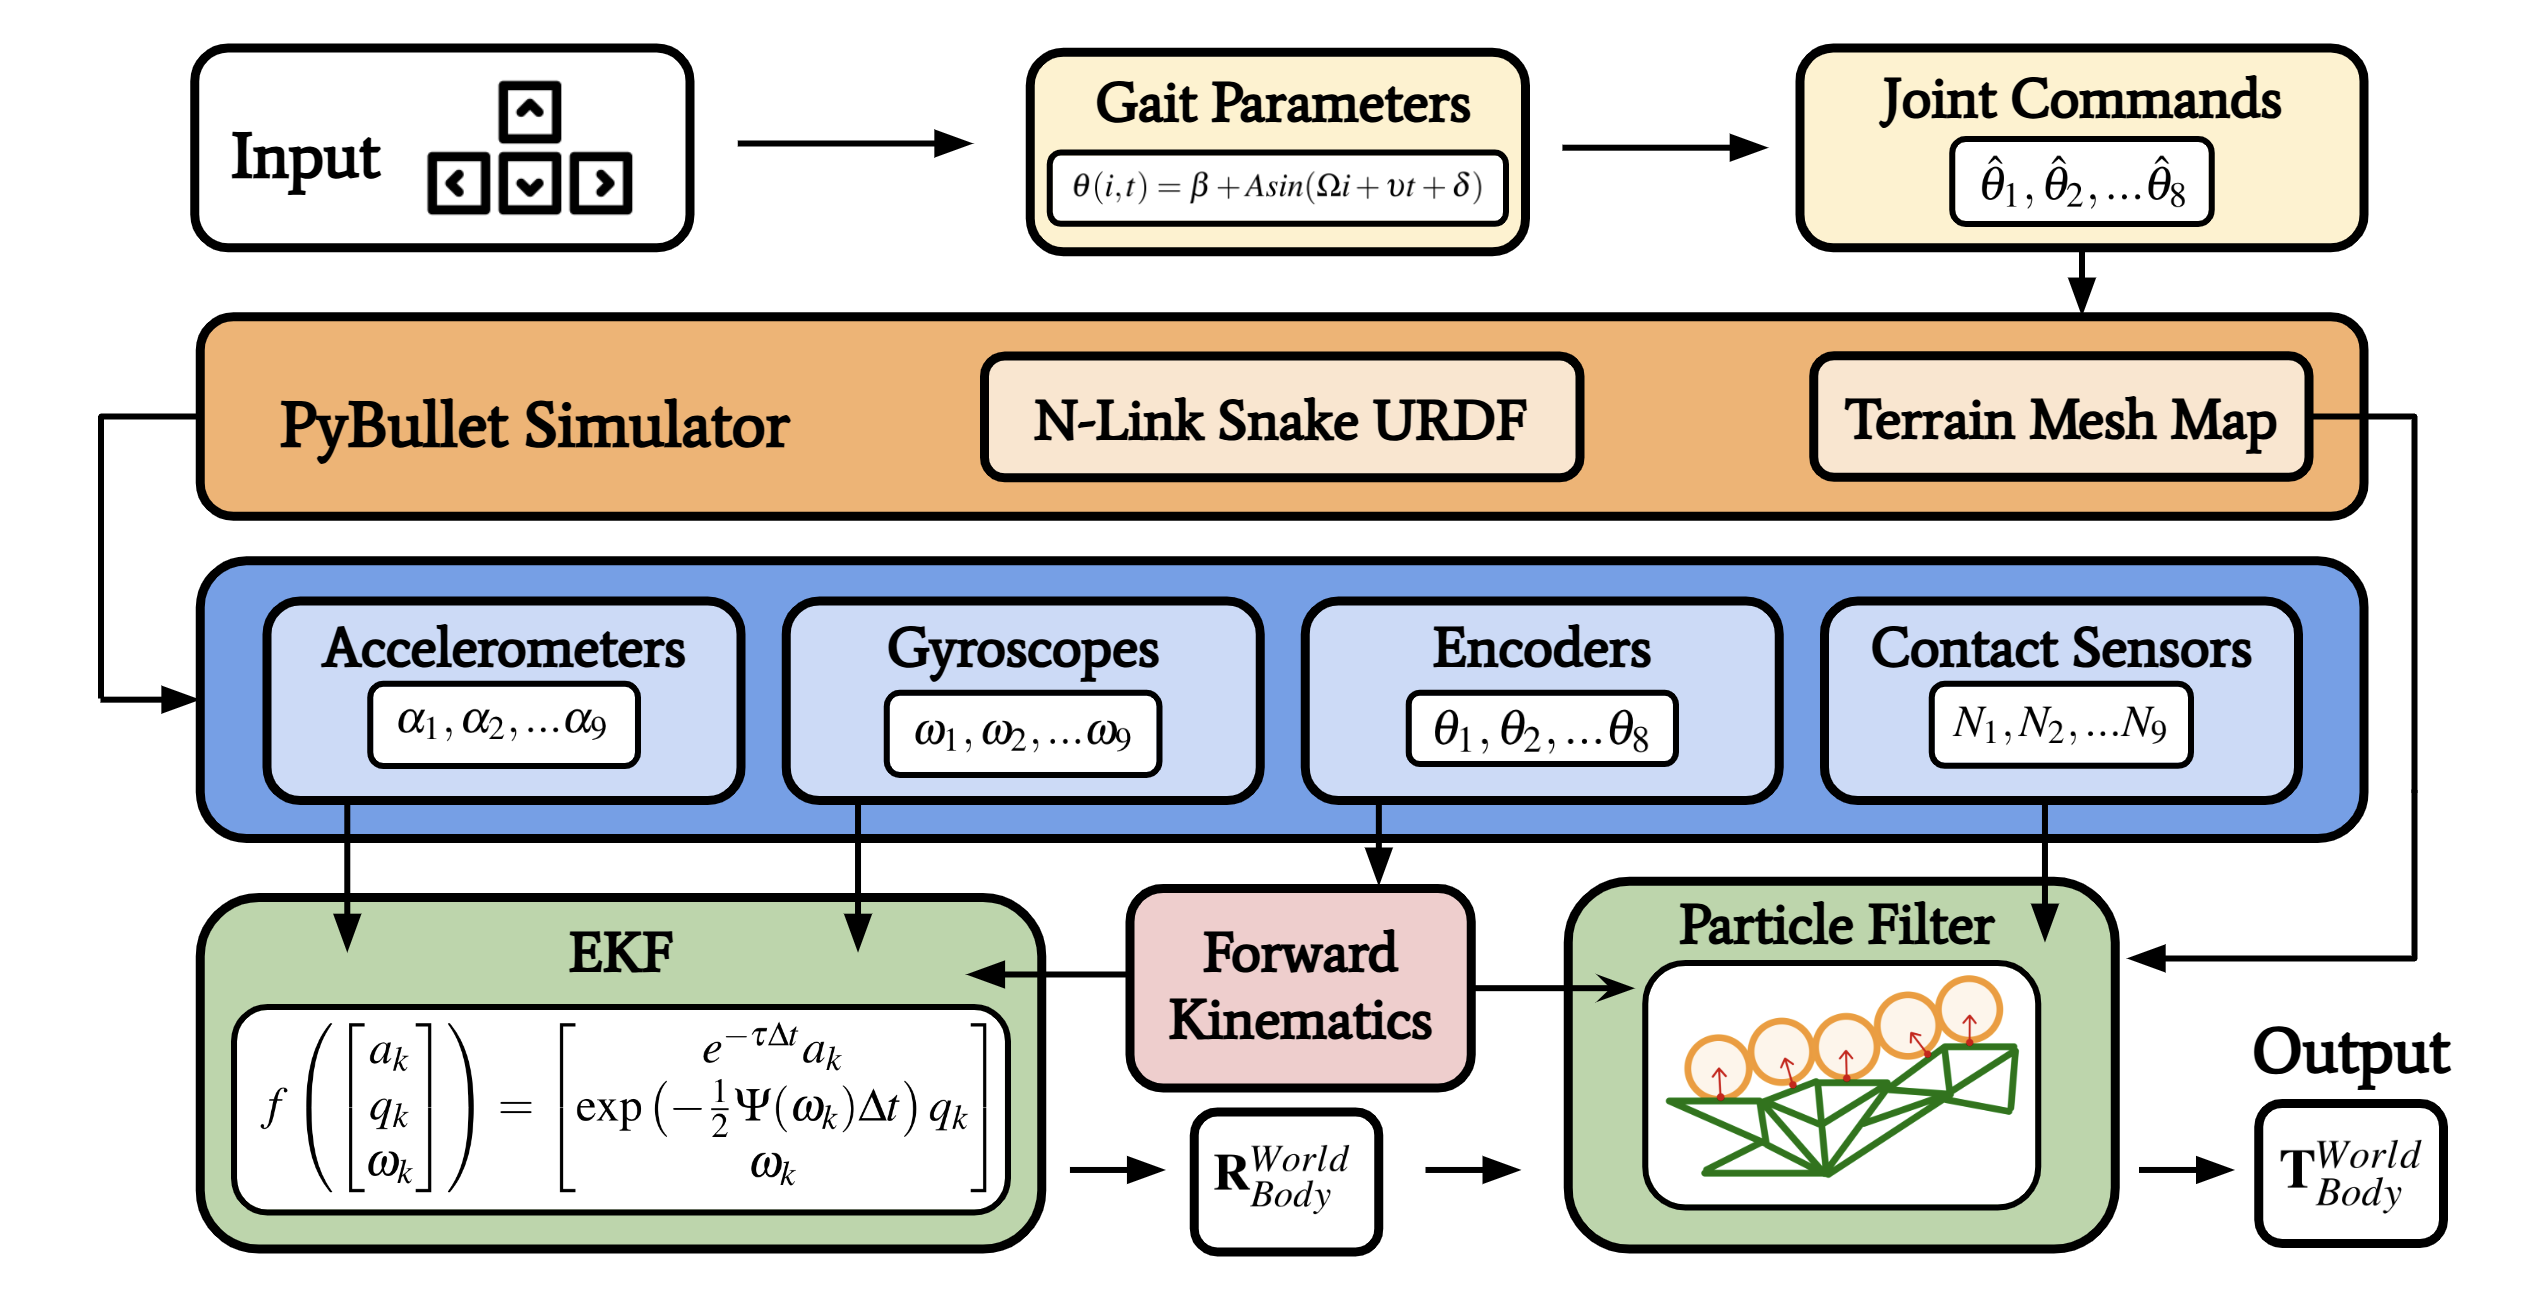
\includegraphics[scale=0.3]{diagram.png}
\caption{System diagram of our simulation and estimation pipeline. }
\label{extended_model_arch}
\end{figure*}


\noindent \textbf{The ``Virtual" Body Frame} \\
The "virtual" body frame, as seen in Fig. \ref{fig:snake_overview}, is a dynamic frame that intuitively represents the motion and position of the snake robot. This frame is located at the center of mass of the robot and is rotated to align with the principle moments of inertia of the body. The first step of determining the pose of the "virtual" body frame is to find the geometric center of mass ($\Bar{x}$, $\Bar{y}$, $\Bar{z}$) of the robot in the initial snake-head frame using forward kinematics. We can then subtract the center of mass of each link from its position in the head frame to construct the 9x3 matrix $\mathcal{P}$ below. 


\begin{equation}
    \mathcal{P} = USV^T = \begin{bmatrix}
        x_1 - \Bar{x} & y_1 - \Bar{y} & z_1 - \Bar{z} \\
        x_2 - \Bar{x} & y_2 - \Bar{y} & z_2 - \Bar{z} \\
        & ... &  \\
        x_9 - \Bar{x} & y_9 - \Bar{y} & z_9 - \Bar{z} \\
    \end{bmatrix}
\end{equation}

As shown above, we next perform singular value decomposition on $\mathcal{P}$ following [\cite{virtual_chas}]. The matrix $V$ serves as a rotation matrix describing the orientation of the coordinate frame aligned with the principle moments of inertia, described in the snake-head frame. By combining the rotation matrix, $V$, with the center of mass, we can establish the virtual chassis frame with respect to the snake-head frame. 

\subsection{Extended Kalman Filter}
To estimate the orientation of the snake robot's body frame (the virtual chassis frame defined above) with respect to an inertial frame, we use an Extended Kalman Filter (EKF) adapted from \cite{state_est_snake_robots}. The state vector of the EKF includes the orientation, acceleration, and angular velocity of the body frame with respect to the inertial frame:
\begin{equation}
    \mathbf{x}_k = \begin{bmatrix}
        a_k & q_k & \omega_k
    \end{bmatrix}^\top \in \mathbb{R}^{10}
\end{equation}



Where $a_k$ is the acceleration of the body frame, $q_k$ is the quaternion representing the orientation of the body frame, and $\omega_k$ is the angular velocity of the body frame. The joint angles and joint angular velocities were not included in the state vector (in contrast to the formulation from \cite{snake_paper2}) because our simulated absolute encoders did not suffer from the same reliability issues as those used in \cite{snake_paper2}. This also had the benefit of simplifying the update step and increasing the efficiency of the filter. \\

\noindent \textbf{Prediction Step}

The prediction step of the EKF uses an autonomous process model that simply propagates the state forward in time using the kinematic equations of motion, under the assumptions of constant angular velocity and additive gaussian noise:
\begin{align}
\mathbf{x}_{k+1} &= f(\mathbf{x}_k) + \mathbf{w}_k, \quad \mathbf{w}_k \sim \mathcal{N}(0, Q) \\
f\left(\begin{bmatrix}
    a_k \\ q_k \\ \omega_k
\end{bmatrix}\right) &= \begin{bmatrix}
    e^{-\tau \Delta t} a_k \\
    \exp\left(-\frac{1}{2} \Psi(\omega_k) \Delta t\right) q_k \\
    \omega_k
\end{bmatrix}
\end{align} 
Where $\tau$ is an acceleration damping factor necessary to maintain stability, $\Delta t$ is the time step between prediction steps, and $\Psi(\omega) \in \mathbb{R}^{4 \times 4}$ is the skew-symmetric matrix of angular velocities used to compute the quaternion derivative. The process noise $\mathbf{w}_k$ is assumed to be zero-mean gaussian with constant covariance $Q$. 

The state covariance matrix $P_k$ is then updated according to the standard EKF prediction equations, using the Jacobian of the process model:
\begin{align}
    P_{k+1} &= F_k P_k F_k^\top + Q \\
    F_k &= \pd{f}{\mathbf{x}_k} = \begin{bmatrix}
        I e^{-\tau \Delta t} & 0 & 0 \\
        0 & \pd{q_{k+1}}{q_k} & \pd{q_{k+1}}{\omega_k} \\
        0 & 0 & I
    \end{bmatrix}
\end{align}

\noindent \textbf{Correction Step}

The correction step of the EKF uses the IMU and encoder measurements from each link of the snake to update the state estimate. The measurement at time $k$ is given by:
\begin{align}
    \mathbf{z}_k &= \begin{bmatrix}
        \bm{\alpha}_k & \bm{\gamma}_k
    \end{bmatrix}^\top \in \mathbb{R}^{6N+1} \\
    \bm{\alpha}_k &= \begin{bmatrix}
        \alpha_k^1 \\ \vdots \\ \alpha_k^{N+1}
    \end{bmatrix}, \quad \bm{\gamma}_k = \begin{bmatrix}
        \gamma_k^1 \\ \vdots \\ \gamma_k^{N+1}
    \end{bmatrix} \\
    \alpha_k^i &= \begin{bmatrix}
        \alpha_x^i \\ \alpha_y^i \\ \alpha_z^i
    \end{bmatrix}, \quad \gamma_k^i = \begin{bmatrix}
        \gamma_x^i \\ \gamma_y^i \\ \gamma_z^i
    \end{bmatrix}
\end{align}
Where $\alpha_k^i$ and $\gamma_k^i$ are the accelerometer and gyroscope measurements, respectively, from link $i$ at time $k$ expressed in the link frame. While the encoder measurements are used in the correction step, they are not included in the measurement vector and measurement model because they are assumed to have negligible noise and cannot be predicted from the state vector.

The measurement model maps the inertial state of the robot's virtual chassis frame to the inertial state of each link. This means it is a function of both the forward kinematic equations and the transform that defines the virtual chassis frame relative to the snake head frame. The measurement model is given by:
\begin{align}
    \hat{\mathbf{z}}_k &= h(\mathbf{x}_k) + \mathbf{v}_k = \begin{bmatrix}
        \hat{\alpha}_k^1 \\ \vdots \\ \hat{\alpha}_k^{N+1} \\ \hat{\gamma}_k^1 \\ \vdots \\ \hat{\gamma}_k^{N+1}
    \end{bmatrix} + \mathbf{v}_k, \quad \mathbf{v}_k \sim \mathcal{N}(0, R) \\
    \hat{\alpha}_k^i &= (W_k^i)^\top R_k^\top (g + a_k) + \hat{a}_{\text{internal}}^i \\
    \hat{\gamma}_k^i &= (W_k^i)^\top \omega_k + \hat{\omega}_{\text{internal}}^i
\end{align}

Where $W_k^i$ is the rotation matrix from link $i$ to the virtual chassis frame at time $k$, $R_k$ is the rotation matrix from the virtual chassis frame to the world frame at time $k$, $g$ is the vector of acceleration due to gravity, and $\hat{a}_{\text{internal}}^i$ and $\hat{\omega}_{\text{internal}}^i$ are respectively the predicted acceleration and angular velocity of link $i$ relative to the virtual chassis frame. Note that $R_k$ is computed by simply converting the quaternion $q_k$ to a rotation matrix, and therefore represents the same orientation estimated by the EKF.

To compute $\hat{a}_{\text{internal}}^i$, the second derivative of the position of link $i$ relative to the virtual chassis frame is approximated by finite differencing across three time steps:
\begin{align}
    \hat{a}_{\text{internal}}^i &= \frac{p_k^i - 2p_{k-1}^i + p_{k-2}^i}{\Delta t^2}
\end{align}
Where $p_k^i$ is the position of link $i$ relative to the virtual chassis frame at time $k$. Similarly, $\hat{\omega}_{\text{internal}}^i$ is approximated by finite differencing $W_k^i$ across two time steps. This computation can be represented simply using the $SO(3)$ logarithm and vee $(\cdot)^\vee$ operators:
\begin{equation}
    \hat{\omega}_{\text{internal}}^i \approx \frac{\log\left((W_k^i)^\top W_{k-1}^i\right)^\vee}{\Delta t}
\end{equation}

Using this measurement model, the state estimate is then updated according to the standard EKF correction equations:
\begin{align}
    K_k &= P_k H_k^\top (H_k P_k H_k^\top + R)^{-1} \\
    \mathbf{x}_{k+1} &= \mathbf{x}_k + K_k(\mathbf{z}_k - \hat{\mathbf{z}}_k) \\
    P_{k+1} &= (I - K_k H_k) P_k \\
    H_k &= \pd{h}{\mathbf{x}_k} = \begin{bmatrix}
        \pd{\hat{\alpha}_k^1}{a_k} & \pd{\hat{\alpha}_k^1}{q_k} & \pd{\hat{\alpha}_k^1}{\omega_k} \\
        \vdots & \vdots & \vdots \\
        \pd{\hat{\alpha}_k^{N+1}}{a_k} & \pd{\hat{\alpha}_k^{N+1}}{q_k} & \pd{\hat{\alpha}_k^{N+1}}{\omega_k} \\
        \pd{\hat{\gamma}_k^1}{a_k} & \pd{\hat{\gamma}_k^1}{q_k} & \pd{\hat{\gamma}_k^1}{\omega_k} \\
        \vdots & \vdots & \vdots \\
        \pd{\hat{\gamma}_k^{N+1}}{a_k} & \pd{\hat{\gamma}_k^{N+1}}{q_k} & \pd{\hat{\gamma}_k^{N+1}}{\omega_k}
    \end{bmatrix}
\end{align}
Computation of the Jacobian $H_k$ can be simplified by solving for the individual partial derivatives symbolically and then constructing the matrix:
\begin{align}
    \pd{\hat{\alpha}_k^i}{a_k} &= (W_k^i)^\top R_k^\top, \quad
    \pd{\hat{\alpha}_k^i}{q_k^j} = (W_k^i)^\top \left(\pd{R_k}{q_j}\right)^\top (g + a_k) \\
    \pd{\hat{\alpha}_k^i}{\omega_k} &= 0, \quad
    \pd{\hat{\gamma}_k^i}{a_k} = 0, \quad
    \pd{\hat{\gamma}_k^i}{q_k} = 0 \\
    \pd{\hat{\gamma}_k^i}{\omega_k} &= (W_k^i)^\top
\end{align}

As a final part of the correction step, the quaternion $q_k$ is normalized to ensure that it remains a valid rotation, since this condition is not maintained by the ordinary EKF equations. While this is not a fully correct or optimal solution, it has been shown to generally work well in practice.

\subsection{Particle Filter}

A particle filter is used to estimate the final pose of the virtual body. Each particle $\mathbf{P}_i$ represents a simulated instance of our snake robot with a pose and non-negative weight:

\begin{align}
    \mathbf{P}_i &= (T^{Body}_{World} \in SE(3), w \in \mathbb{R}^+)
\end{align}

\noindent \textbf{Action Model}

\noindent Before the prediction step, the $SO(3)$ orientation of each particle is fixed to the output of the EKF. The action model is defined as perturbing each particle's pose by a random walk model proportional to the commanded twist magnitude. The perturbation is represented by a tangent element $\tau \in \mathbb{R}^6$. Each component is clipped to a range to ensure particle diversity in directions that are not currently being moved in.

\begin{align}
    T_{new} &= T_{old} * \exp(\tau_{clipped} * |\tau_{command}|)
    \\
    \tau_{clipped} &= \text{clip}(\tau_{sample}, \tau_{min}, \tau_{max})
    \\
    \quad \tau_{sample} &\sim \mathcal{N}(0, I) \in \mathbb{R}^6
\end{align}

\noindent \textbf{Sensor Model}

\noindent The snake is operating in a terrain with known height values. We can pre-compute a normal map using PyBullet by shooting a ray down from the sky onto the surface. We assume a convex surface laterally - caves, alcoves, and similar features that dig into vertical walls are not allowed. Therefore each ray is guaranteed to strike the terrain with a returned normal vector. We can readily compare these values to the normal vectors provided by our exteroceptive contact sensors.

When we receive an update $(i, N_{sensor} \in \mathbb{R}^3)$ where $i$ is a joint index, we can iterate over each particle and see how well its pose aligns with the new sensor data. We compute the pose $T^{joint}_{world}$ for the corresponding simulated link. The $x$ and $y$ components are then used to lookup the expected normal $N_{particle}$ based on the terrain. We can then update the weights accordingly:

\begin{align}
    w_{new} = w_{old} * \frac{N_{particle} \cdot N_{sensor} + 1 }{2}
\end{align}

\noindent \textbf{Final Estimate}

\noindent The final pose estimate is the EKF orientation concatenated with the weighted average of each particle's position.

\subsection{Pybullet Simulation Environment}
To implement and test our EKF and particle filter estimation mechanisms, our team decided to use the Pybullet physics engine \cite{pybullet}. We started by implementing the snake robot itself in simulation with actuated revolute joints with position control. A nice feature of this simulator is its direct modeling of anisotropic friction coefficients that are essential for locomoting the snake. Our team also implemented a randomized terrain mesh directly in Pybullet for simulating the snake's gaits in complex environments. 

We also wrote various modules in our codebase to simulate different sensors required by our robot including accelerometers, gyros, and force-contact sensors. The simulated accelerometer measurements required differentiating given body velocities numerically.  


\section{Results}
To evaluate our system, we validated the performance of the EKF and particle filter separately. The following section details the results of our method.

\subsection{EKF}
The output of the EKF is the orientation of the body frame with respect to the world frame. To test the correctness of our implementation, we first tested the behavior of the prediction step.

\begin{figure}[H]
    \centering
    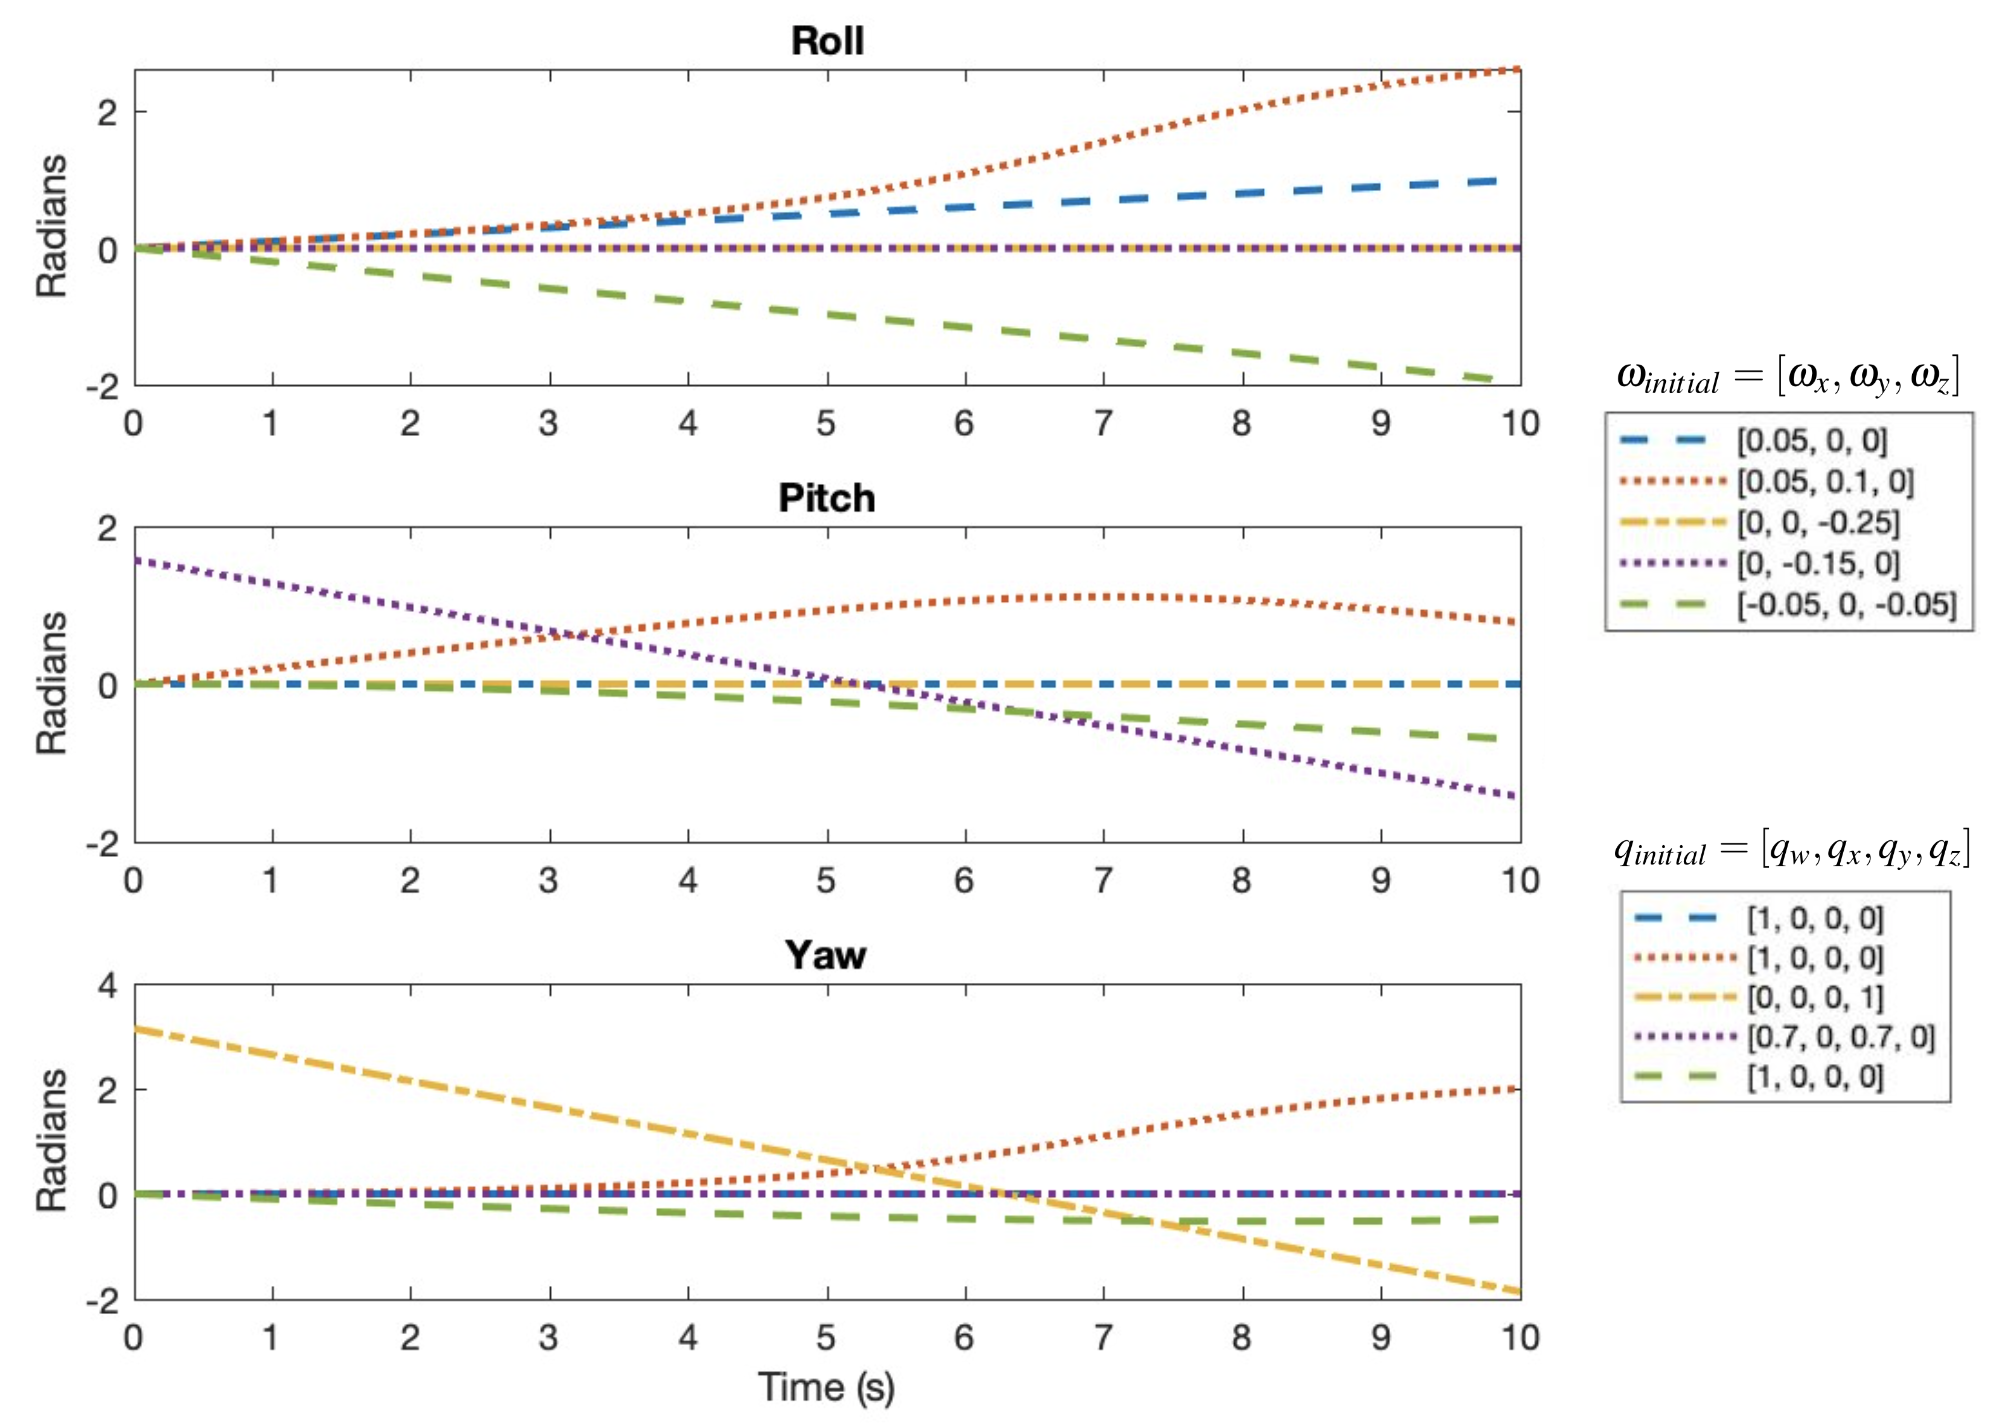
\includegraphics[width = 0.85\linewidth]{ekf_predict.png}
    \caption{EKF prediction trajectories in roll, pitch, and yaw, for different initial angular velocities ($\omega$), rotations ($q$), and zero acceleration ($\alpha=0$)}
    \label{fig:ekf_predict}
\end{figure}

Figure \ref{fig:ekf_predict} shows the orientation trajectories for different initial rotations and angular velocities. for a more intuitive understanding of these trajectories, the quaternion orientation is converted into roll, pitch, and yaw. The blue line has a constant angular velocity of $\omega_x$ in the x direction which results in the pitch and yaw remaining constant, while the frame rotates about the x axis (roll). For the red line, with positive angular velocities $\omega_x$ and $\omega_y$, the roll and pitch increase until around 6 seconds and then the roll and yaw begin to increase faster while the pitch flattens out. Both of these cases, as well as with all others we tested align with the behavior we would expect for the predict step.\\

To test the update step of the EKF, we started by looking at the behavior for when the snake is simply moving in a straight line. Because the shape of the snake isn't changing while it does the "inchworm" motion forward, we would expect the EKF output to maintain a constant orientation. Figure \ref{fig:ekf_quaternion_sad} shows the output of the estimated quaternion of the virtual body frame versus the ground truth virtual body frame. As seen in this figure, the EKF output is very off from the ground truth, and we can see oscillatory behavior where the quaternion estimate is going back and forth between two incorrect estimates.

\begin{figure}[H]
    \centering
    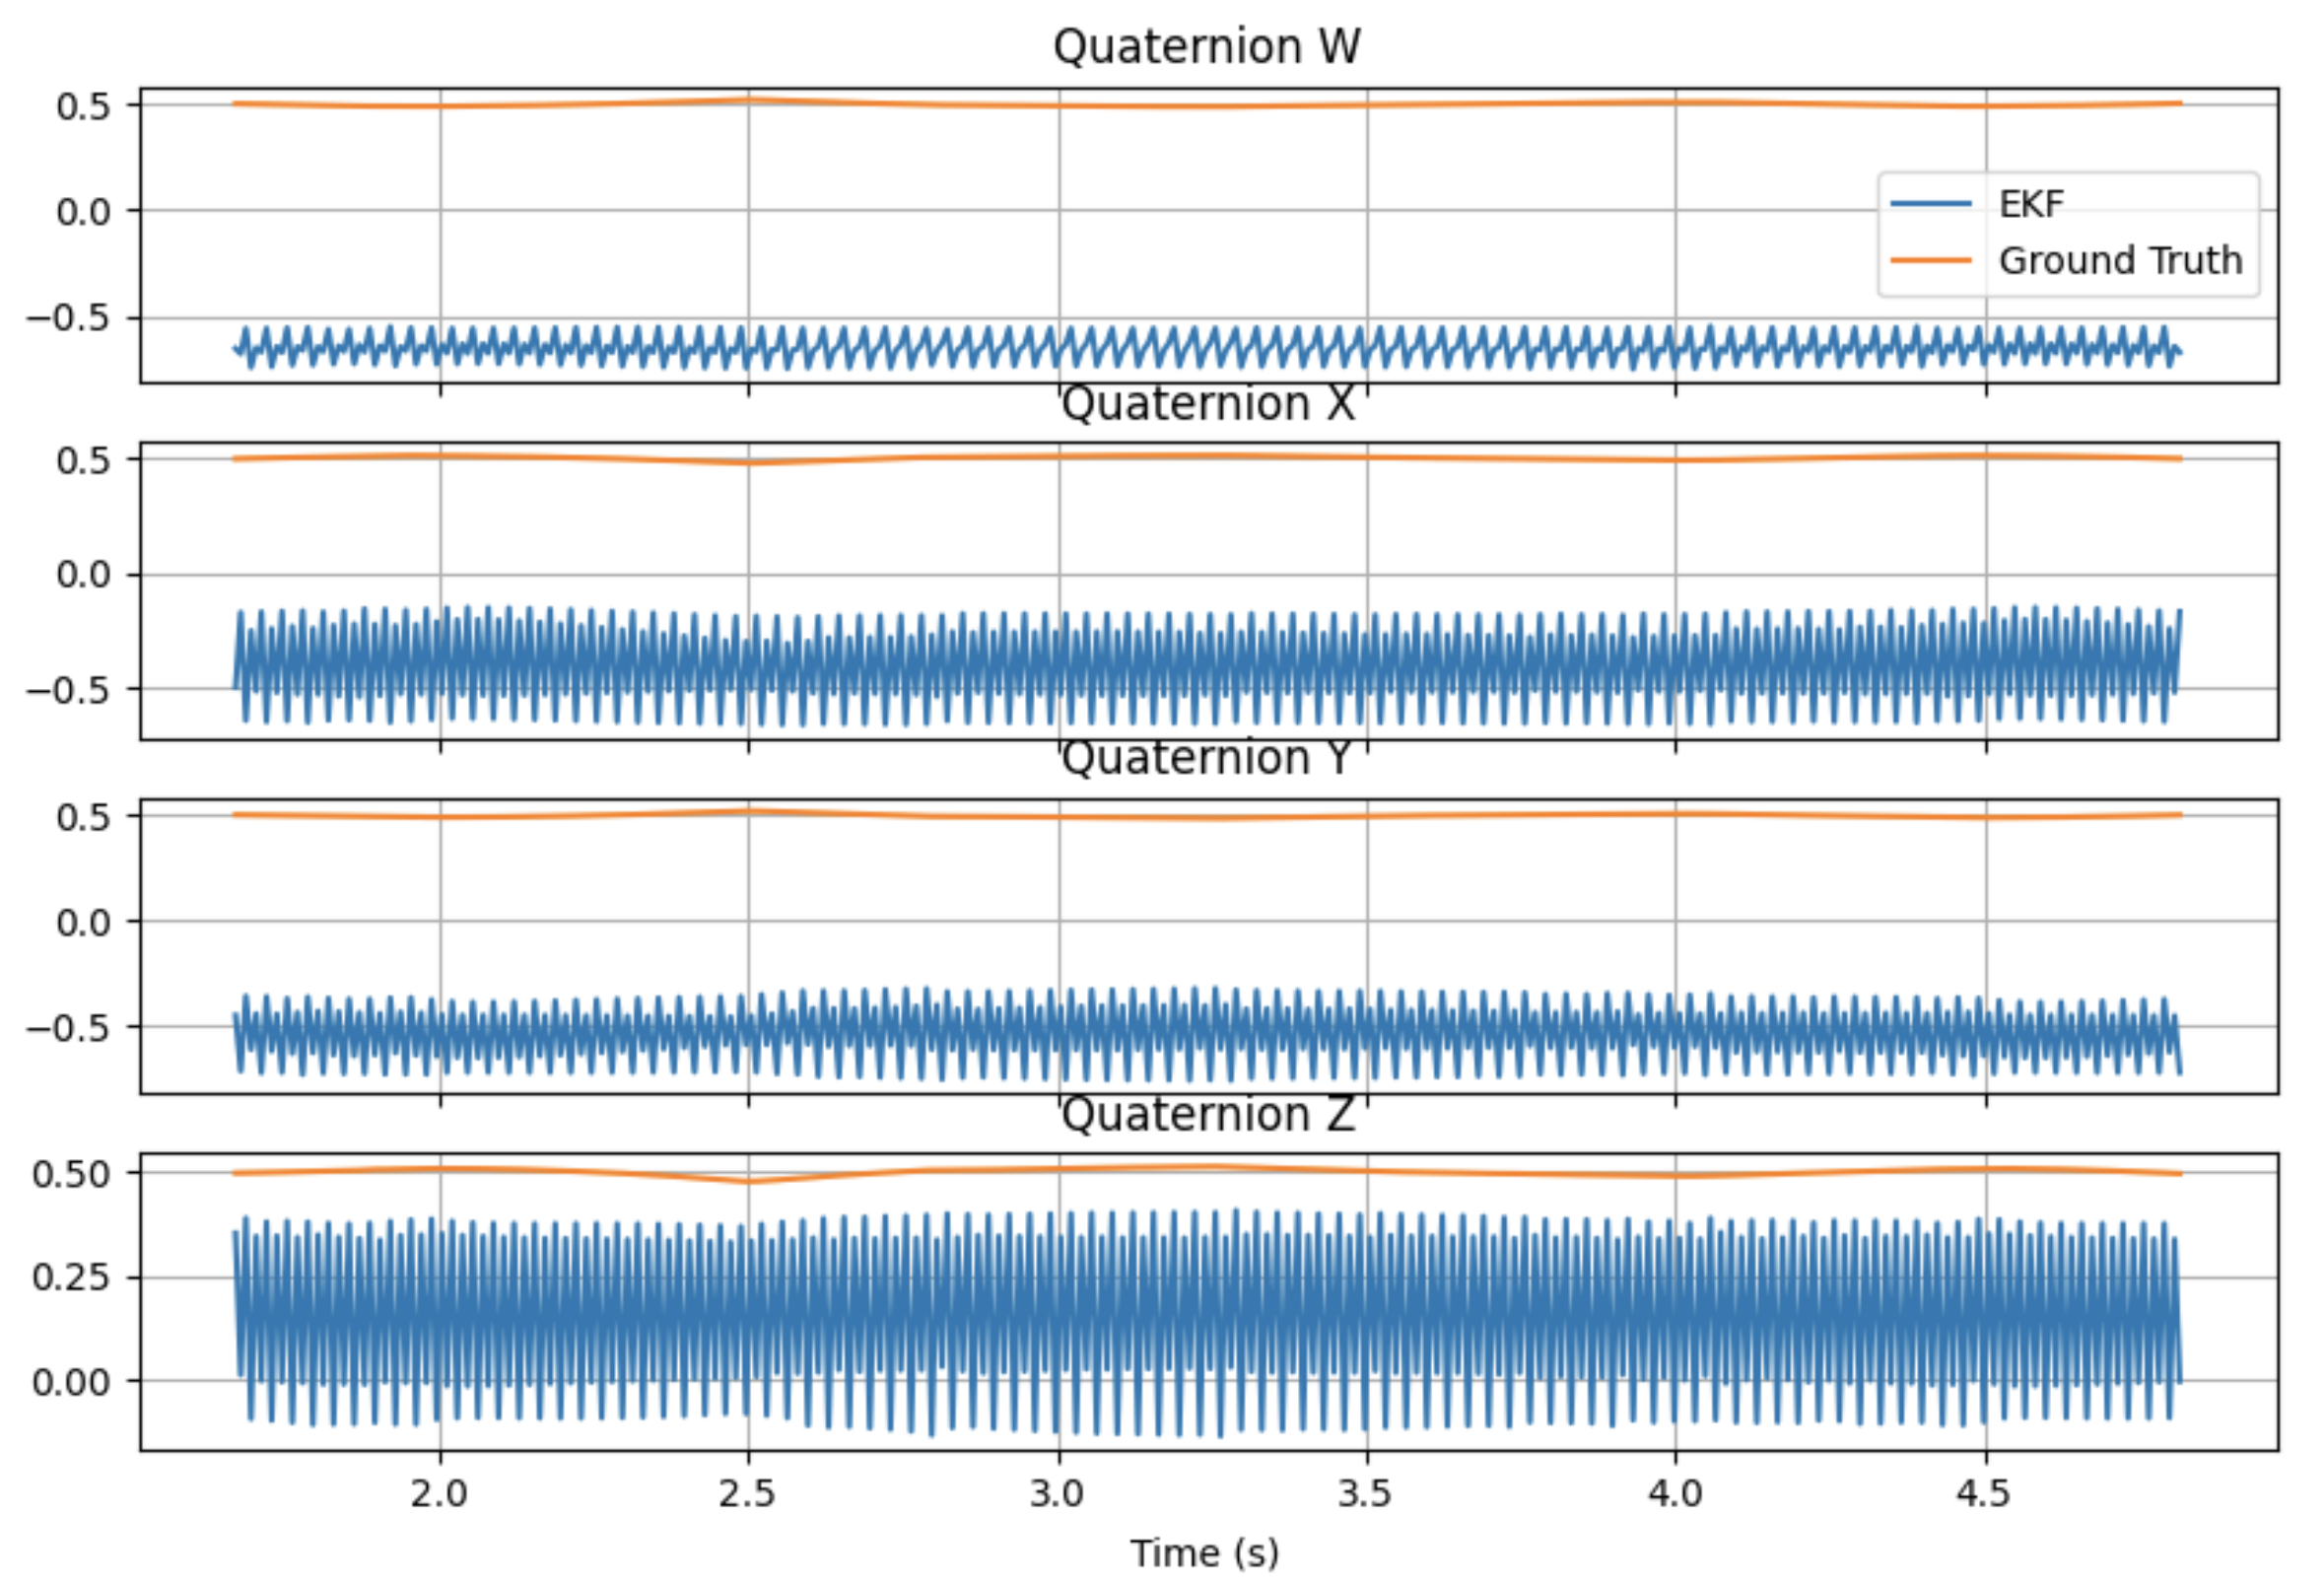
\includegraphics[width = 0.75\linewidth]{ekf_update_sad.png}
    \caption{Ground Truth vs. EKF Estimate for Quaternion Orientation when snake is performing the "inchworm" gait.}
    \label{fig:ekf_quaternion_sad}
\end{figure}

To investigate this issue further our group focused on comparing the simulated IMU measurements versus our predicted IMU measurements. 

\begin{figure}[H]
    \centering
    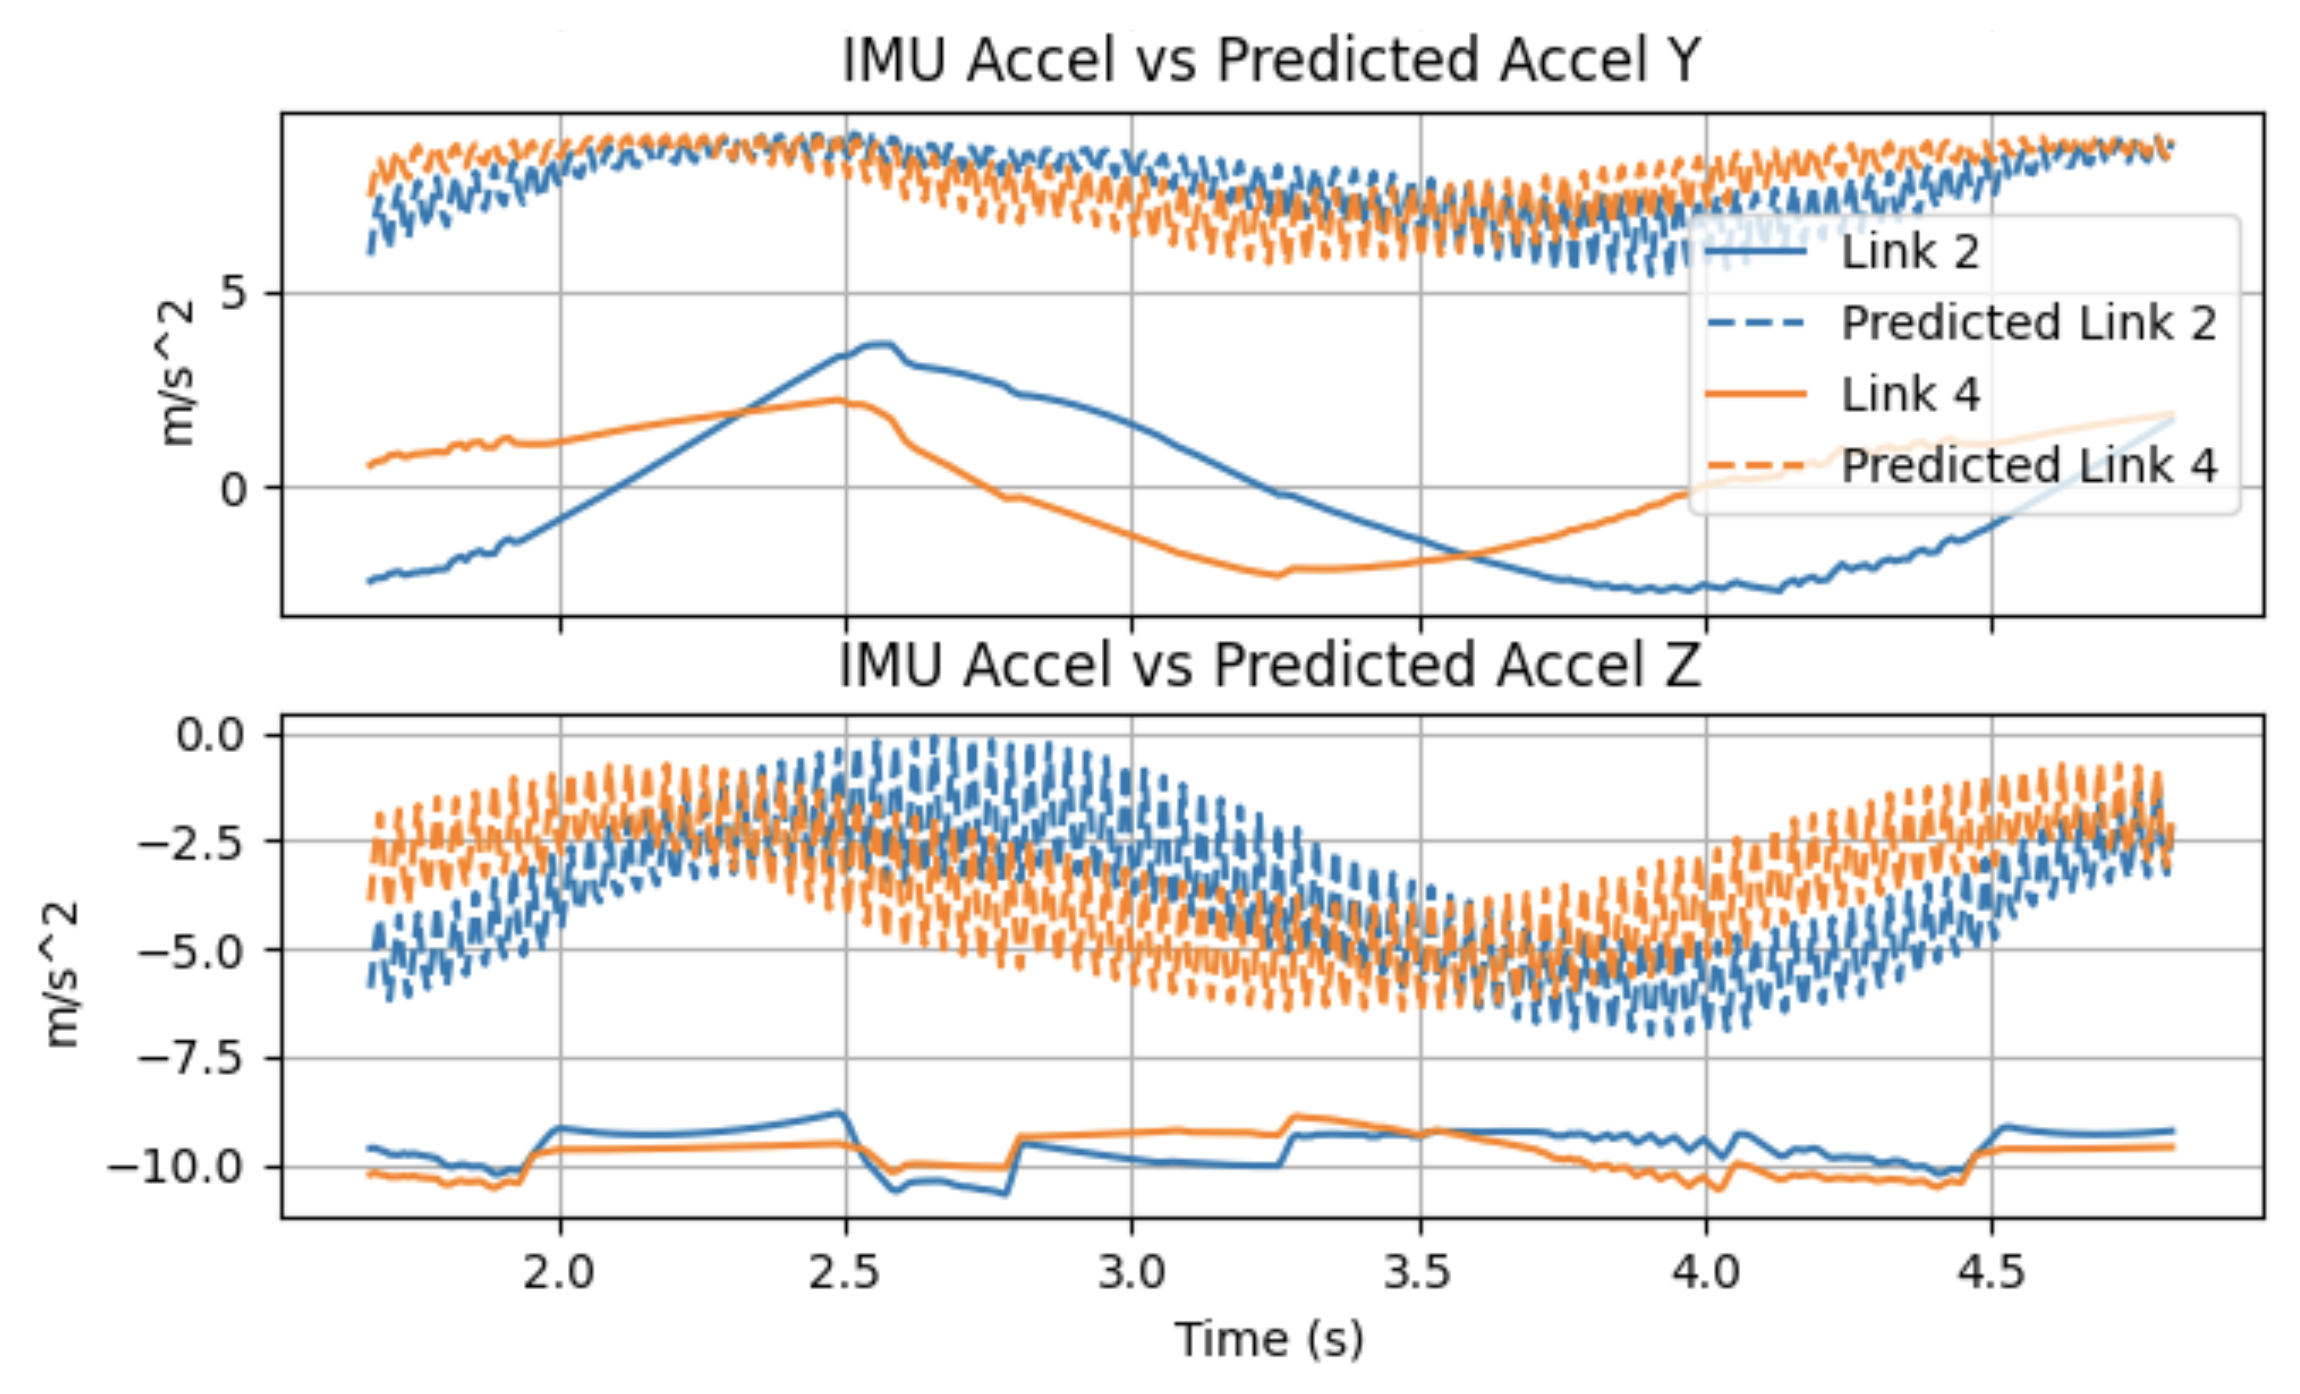
\includegraphics[width = 0.75\linewidth]{ekf_bad_accels.png}
    \caption{IMU accelerometer readings vs. EKF predicted accelerometer readings when snake is performing the "inchworm" gait.}
    \label{fig:ekf_bad_accels}
\end{figure}

As shown in Figure \ref{fig:ekf_bad_accels}, the EKF predicted accelerations are significantly off from the measured IMU accelerations. The same oscillatory behavior can be seen in the predicted accelerations because the corresponding quaternion for each of the predicted measurements is also oscillating (Figure \ref{fig:ekf_quaternion_sad}). These incorrect predicted acceleration measurements would explain the odd behavior from our EKF update step.\\

To further show the issues in our update step, we used the ground truth orientation of the virtual body frame and input it into the update step to test if our predicted accelerations were aligned.

\begin{figure}[H]
    \centering
    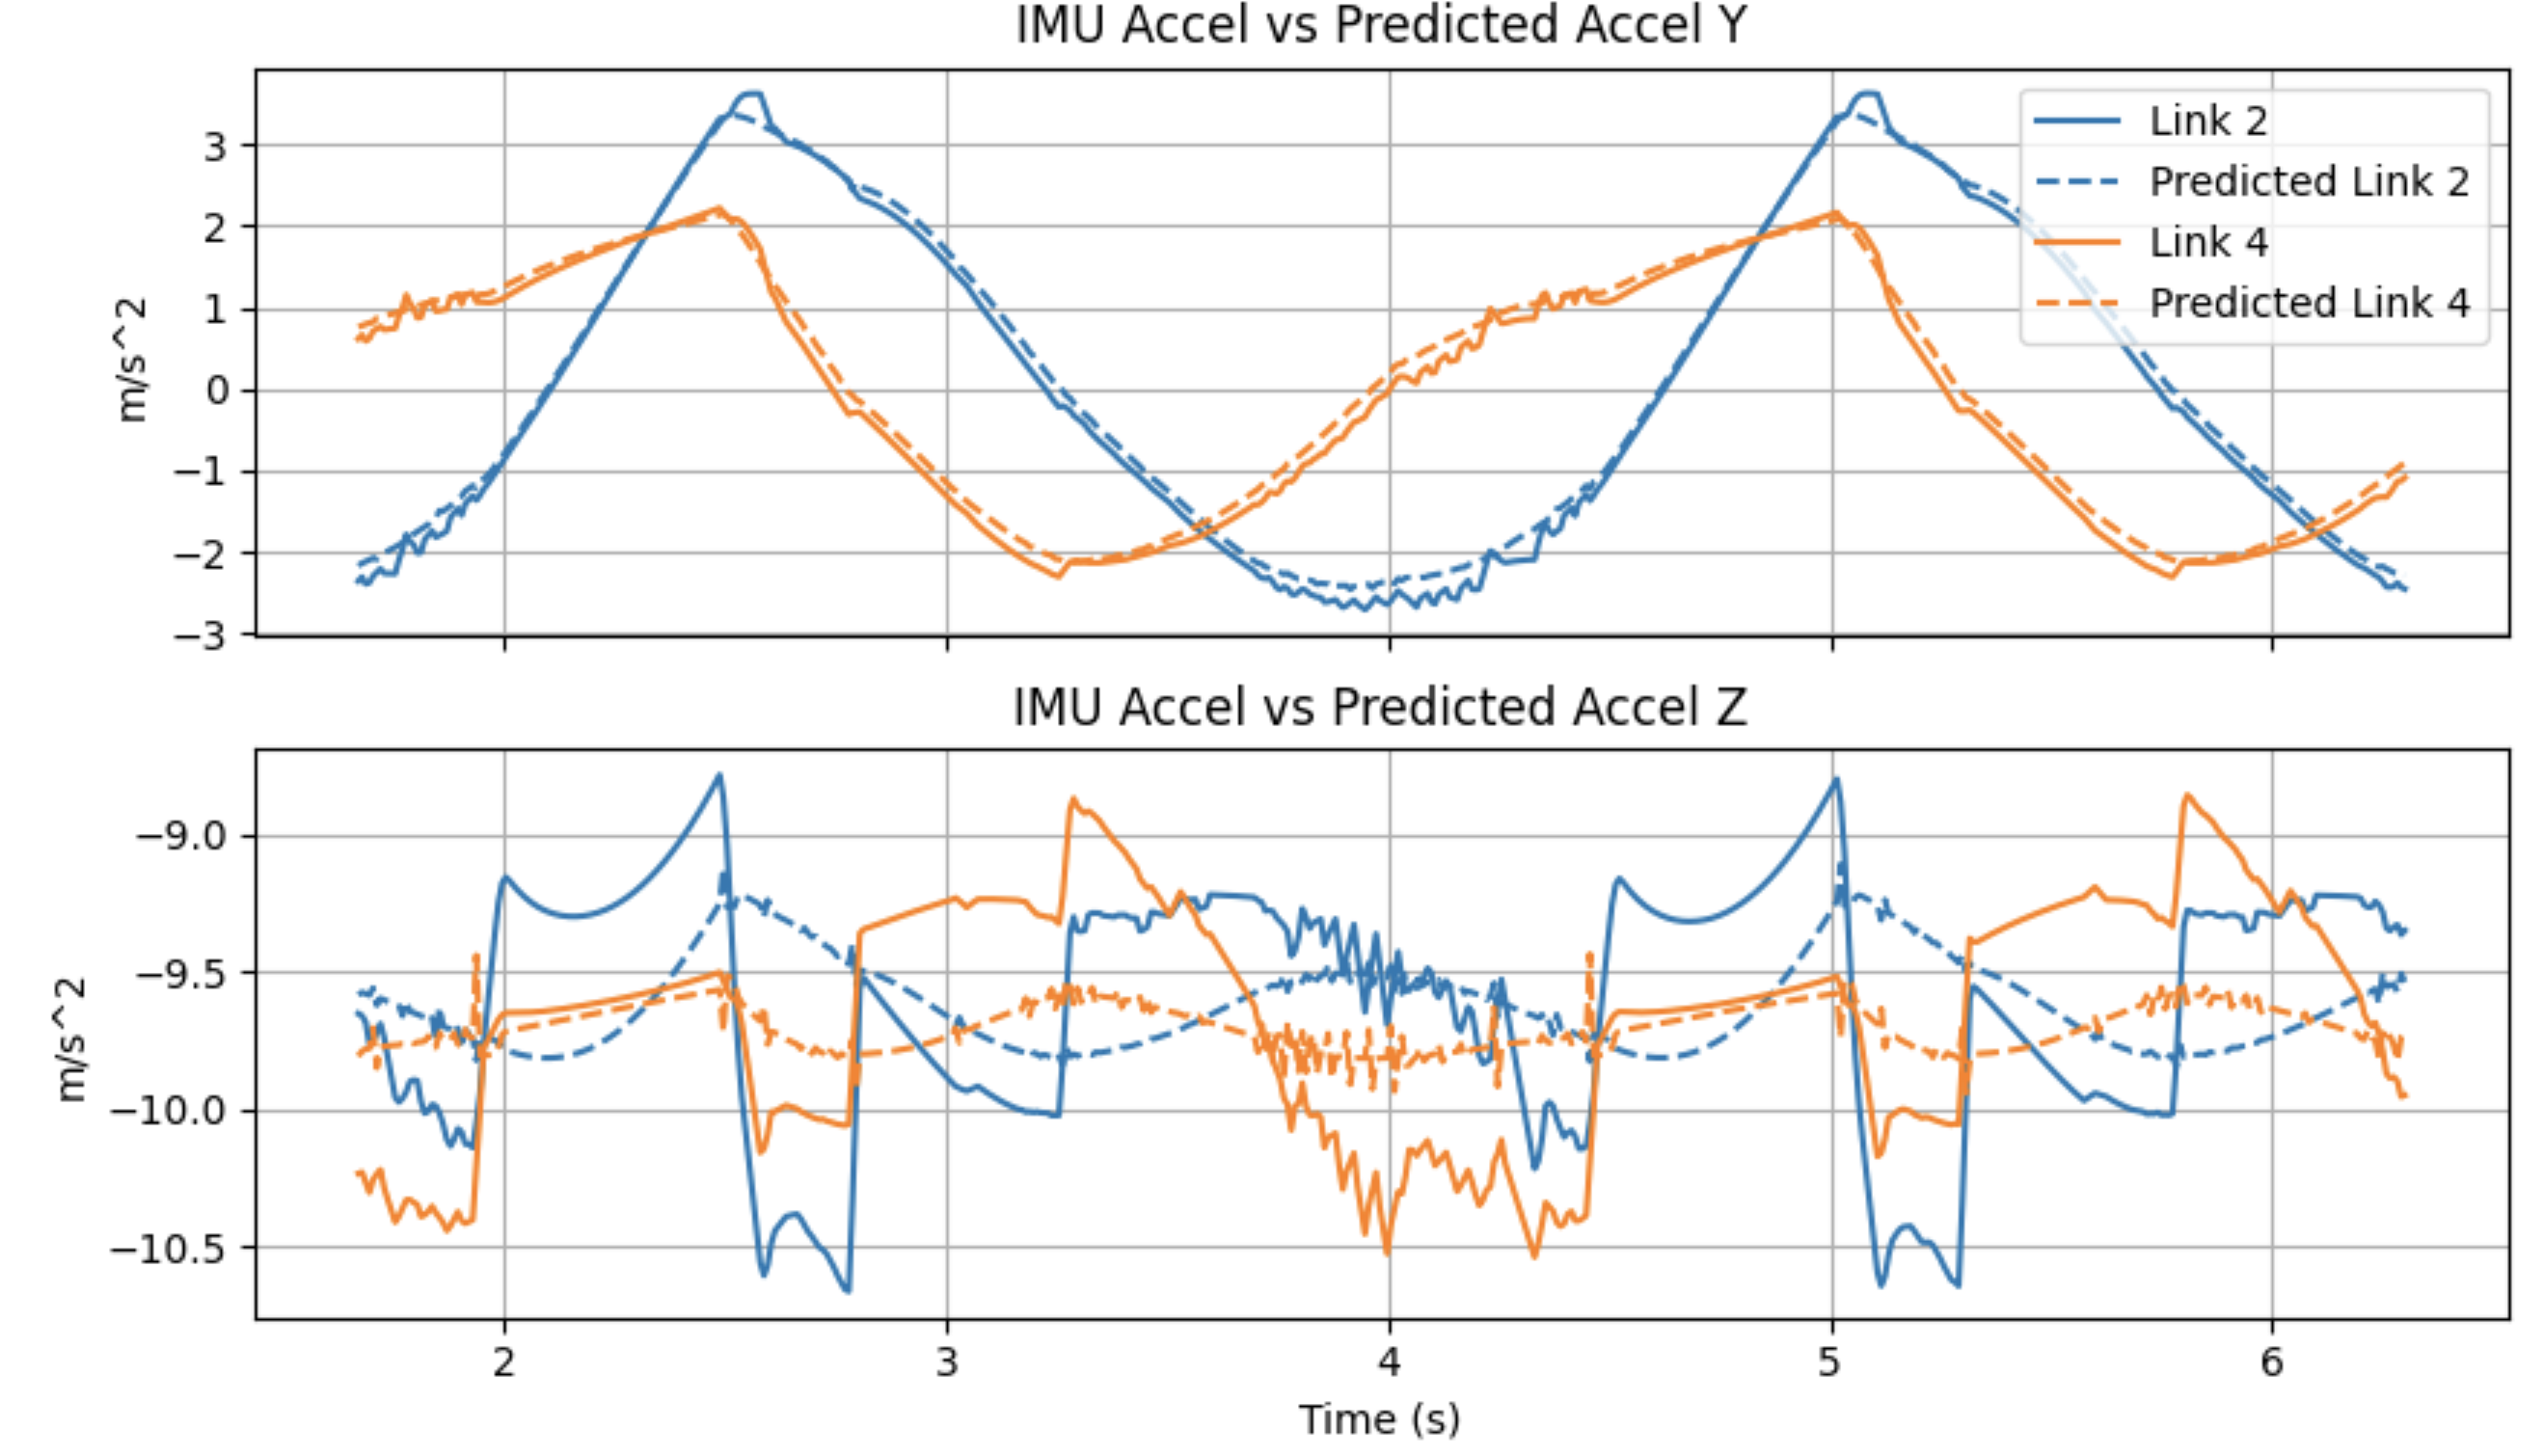
\includegraphics[width = 0.75\linewidth]{ekf_accels_w_gt.png}
    \caption{IMU accelerometer readings vs. EKF predicted accelerometer readings when snake is performing the "inchworm" gait and the update step has ground truth orientation.}
    \label{fig:ekf_accels_w_gt}
\end{figure}

Figure \ref{fig:ekf_accels_w_gt} shows the IMU accelerations versus the predicted EKF accelerations with ground truth orientation. In this case, the Y accelerations are well aligned with each other, but the Z accelerations are still not perfect. If both of these accelerations matched up perfectly with each other, then it would suggest that our jacobians could be incorrect in the update step. However, since we are not sure if the Z prediction step is correct, it could mean that we are computing our prediction wrong. 

One success case our team found was when the snake made a curled, "C" shape. In Figure \ref{fig:ekf_success} we show the estimate quaternion orientation of the snake over time. At t = 0s, the snake starts by being perfectly straight. Here we again see the oscillatory behavior described from above. At t = 1.5s, the snake is curled slightly to the right, and, while the quaternion is still not accurate, the oscillations in the estimated orientation are gone. Finally, at t = 7.75s, the snake is curled to the right once more to make a "C" shape. This results in the quaternion estimate varying greatly until it converges on the actual ground truth at t = 9.5s.
\begin{figure}[H]
    \centering
    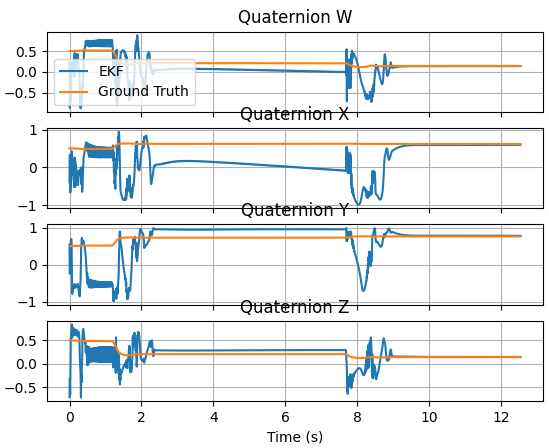
\includegraphics[width = 0.75\linewidth]{quaternion_success_case.png}
    \caption{Ground Truth vs. EKF Quaternion orientation estimate as the snake changes from a straight shape to a curled, "C" shape. }
    \label{fig:ekf_success}
\end{figure}
We believe the EKF successfully converges to the correct orientation only after creating a "C" shape because the IMUs in each link are slightly misaligned with each other which gives the update step more information to correct from.

Although our EKF is able to successfully predict the orientation in some edge cases, we were unable to solve the all the bugs which means our full EKF isn't able to correctly predict the orientation of the virtual body frame for the average case. We leave this as future work to be improved upon.

\subsection{Particle Filter}
Our particle filter is used to estimate the 3D position of the virtual body frame. We compared the ground truth position of the virtual body frame versus the particle filter. For this experiment, we are assuming the EKF produces an accurate orientation of the virtual body frame and thus use the ground truth orientation of the virtual body frame from the simulation.

\begin{figure}[H]
    \centering
    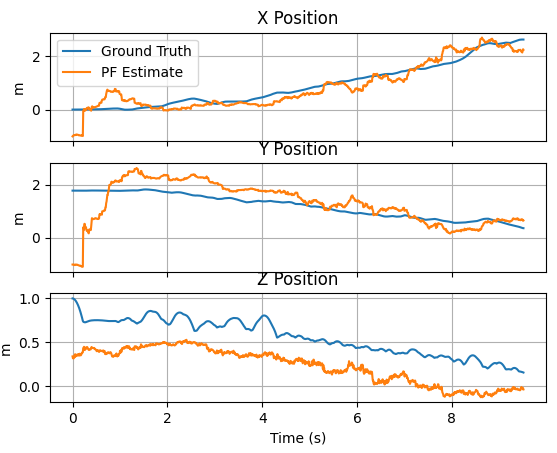
\includegraphics[width = 0.75\linewidth]{pf.png}
    \caption{Particle Filter Position Estimate vs. Ground Truth Virtual Body Frame Position}
    \label{fig:pf_results}
\end{figure}

Figure \ref{fig:pf_results} shows the difference between the ground truth and predicted position of the virtual body frame. For the most part, the particle filter estimate aligns very closely to the ground truth position. There is a slight offset in the z prediction because the particle filter maps the z position to be at a fixed distance above the terrain mesh.


\subsection{Additional Project Deliverables}
For further results, view our project presentation and GitHub which are linked below.\\
\noindent \textbf{Project Presentation}: \href{https://www.youtube.com/watch?v=Mj-DBzjO0Z0}{https://www.youtube.com/watch?v=Mj-DBzjO0Z0}.\\
\noindent \textbf{Project Github}: \href{https://github.com/schefferac2020/SnakeSim}{https://github.com/schefferac2020/SnakeSim}.

\section{Conclusion}
In this work, we presented a hybrid estimation scheme for tracking the shape, orientation, and global position of a 9-link robotic snake. To track the snake's body frame and shape we leveraged the idea of a non-conventional ``virtual chassis frame." We implemented an EKF to estimate the orientation of this virtual chassis frame. Finally, we estimated the global position of the snake by using a particle filter that used the EKF predicted orientation, contact forces, and a terrain map as its inputs. 


\newpage
\printbibliography




\end{document}
